In this section we will go over related work and relevant background information for our model and experiments. The depth of the explanation is adopted to the expected prior knowledge of the reader. The reader is supposed to know the basics of machine learning and deep learning, including probability theory and basic knowledge on neural networks and their different architectures. Basic principles such as forward pass, backpropagation and convolutions are expected to be understood. Further the use and functionality of deep learning modules such as the model, the optimizer and the terms target and prediction should be known. This also includes being familiar with the training and testing pipeline of a model in deep learning.

Should all these boxes be checked, then we can expect to get a deeper understanding of the magic behind the VAE and its differences to a normal autoencoder. After that we will present how convolutional layers can be used on graphs. Of course where there is a layer there is a model, thus we are presenting the graph convolutional network (GCN). Closing the circle we show how we can adopt the VAE to graph convolutions. Wrapping things up, we present the state of the art algorithms for graph matching, which will be util to allow permutation invariance when matching prediction and target graph \cite{paulheim_knowledge_2016}.  


\subsection{Knowledge Graph}

% Knowledge Graphs are great! The best in the world.
% Knowledge Graphs which we will be using
% We will focus on the generation of KGs.
% Representation of KG as adjacency, edge feature and node feature matrix
Knowledge graph has become a popular key phrase. Yet, the term is so broad, that it can have various definitions. In this thesis we are going to focus on KGs in the context of relational machine learning.

% What is a KG
A KG is a database and as all other databases it is used to store data. The main difference to tabular databases is that KGs store data in a relational fashion. A standard KG structure, introduced by the semantic-web community, is the Resource
Description Framework (RDF). It is a so called schema-based approach, meaning that every entity has a unique identifier and all possible relations are stored in a vocabulary. The opposite schema-free approach is used in OpenIE models for information extraction. Here any type of triple can be extracted, eg.  \text{(Michelangelo,  painted,    Sixtine Chapel)}. Where as a triple in RDF format from Freebase, one of the largest open-source KGs, has the form
\begin{equation*}
    (/m/02mjmr, /people/person/born-in, /m/03gh4)
\end{equation*}
%  
\begin{equation*}
    (s, r,  o)
\end{equation*}
 
with:
\begin{itemize}
    \item Subject $s:   /m/02mjmr$ Barack Obama
    \item Relation/Predicate $r:    /people/person/born-in$
    \item Object $o:     /m/03gh4$ Hawaii
\end{itemize}


For all triples $s$ and $o$ are part of a set of so called entities, while $r$ is part of a set of relations. This is enough to define a basic KG.

% Hierarchy, entities, classes
Schema-based KG can include type hierarchies and type constrains. Classes group entities of the same type together, based on common criteria, e.g all names of people can be grouped in the class 'person'. Hierarchies define the inheriting structure of classes and subclasses. Picking up our previous example, 'child' would be a subclass of 'person' and inherit its properties. At the same time the class of an entity can be key to a relation with type constrain, since some relations can only be used in conjunction with entities fulfilling the constraining type criteria.

% Ontology - semantics
These schema based rules of a KG are defined in its ontology. Here properties of classes, subclasses and constrains for relations and many more are defined. Again, we have to differentiate between KGs with open-world or closed-world assumption. In a closed-world assumption all constrains must be sufficiently satisfied before a triple is accepted as valid. This leads to a huge ontology and makes it difficult to expand the KG. On the other hand open-world KGs such as Freebase, accept every triple as valid, as long as it does not violate a constrain. This again leads inevitably to inconsistencies within the KG, yet it is the preferred approach for large KGs. In context of this thesis we refer to the ontology as semantics of a KG, we research if our model can capture the implied closed-world semantics of an open-world KG \cite{nickel_review_2016}.

% Sparse and dense representation
Lastly, we point out one major difference between KGs, namely their representation. RDF KGs are represented as set of triples, consisting of a unique combination of numeric indices. Each index linking to the corresponding entry in the entity and relation vocabulary. This is called dense representation and benefits from fast computation due to an optimized use of memory.

In contrary the dense representation of a triple is the sparse representation. Here a binary square matrix also called the adjacency matrix, indicated a link between two entities. To identify the node, each node in the adjacency matrix has a one-hot encoded entity-vocabulary vector. All one-hot encoded vectors are concatenated to a node attribute matrix.
In simple cases, like citation networks this is a sufficient representation. In the case of Freebase, we need an additional edge-attribute matrix, which indicates the relation  of each link. The main benefits of this method are the representation of subsets of triples, also subgraphs, with more than one relation and the computational possibility to perform graph convolutions. 

% Usecases of KG

% Knowledge graphs have very different formats. The datasets we will be sorting with are in rdf format.
% This format can include an defined onthology or not.
% This means the KG consists of triples subject, relation, object.
% when indexing these triples. we get a dense representation of the KG.
% About sparse KGs

\subsection{Graph VAE – one shot method}

\subsubsection{VAE}
\label{ssection:VAE}
% The VAE as first presented by \cite{kingma_auto-encoding_2014} is an unsupervised generative model consisting of an encoder and a decoder. The architecture of the VAE differs from a common autoencoder by having a stochastic module between encoder and decoder. Instead of directly using the output of the encoder, a distribution of the latent space is predicted from which we sample the input to the decoder. The reparameterization trick allows the model to be differentiable. By placing the sampling module outside the model we get a deterministic model which can be backpropagated.



The VAE as first presented by \cite{kingma_auto-encoding_2014} is an unsupervised generative model in form of an autoencoder, consisting of an encoder and a decoder. Its architecture differs from a common autoencoder by having a stochastic module between encoder and decoder. The encoder can be represented as recognition model with the probability $p_{\boldsymbol{\theta}}(\mathbf{z} \mid x)$ with $x$ being the variable we want to inference and $z$ being the latent representation given an observed value of $x$. The encoder parameters are represented by $\theta$. Similarly, we denote the decoder as $p_{\boldsymbol{\theta}}(\mathbf{x} \mid z)$, which given a latent representation $z$ produces a probability distribution for the possible values, corresponding to the input of $x$. This will be the base architecture of all our models in this thesis.

The main contribution of the VAE is the so called reparameterization trick. When sampling from the latent prior distribution, we get a stochastic module inside our model, which can not be backpropagated and makes learning impossible. By placing the stochastic module outside the model, we can again backpropagate. We use the predicted latent space as mean and variance for a Gaussian normal distribution, from which we then sample $\epsilon$, which acts as external parameter and does not need to be updated.

\begin{figure}[h]
    \centering
    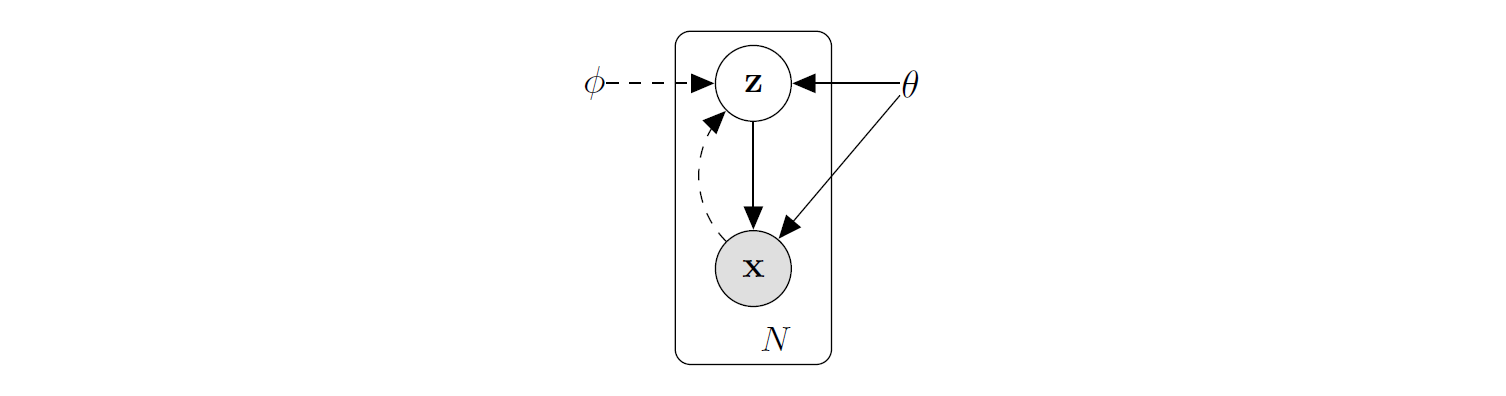
\includegraphics[width=0.75\textwidth]{data/images/repaTrick.png}
    \label{fig:simonGVAE}
    \caption{Representation of the VAE as bayesian network, with solid lines denoting the generator $p_{\boldsymbol{\theta}}(z)p_{\boldsymbol{\theta}}(\mathbf{x} \mid z)$ and the dashed lines the posterior approximation $q_{\phi}(\mathbf{z} \mid \mathbf{x})$ \cite{kingma_auto-encoding_2014}.}
    \label{fig:varinference}
\end{figure}

In \ref{fig:varinference} we see, that the true posterior $p_{\boldsymbol{\theta}}(\mathbf{z} \mid \mathbf{x})$ is intractable. Thus, we make the assumption that the prior to the decoder is Gaussian with an approximately diagonal covariance, which gives us the approximated posterior.

\begin{equation}
    \log q_{\phi}\left(\mathbf{z} \mid \mathbf{x}^{(i)}\right)=\log \mathcal{N}\left(\mathbf{z} ; \boldsymbol{\mu}^{(i)}, \boldsymbol{\sigma}^{2(i)} \mathbf{I}\right)
\end{equation}
    
Now variational inference can be performed, which allows both $\theta$ the generative and $\phi$ the variational parameters to be learned jointly. Using the Monte Carlo estimation of $q_{\phi}(\mathbf{z} \mid \mathbf{x})$ we get the so called estimated lower bound (ELBO):
\begin{equation}
    y_{k}(\mathbf{x}, \mathbf{w})=\sigma\left(\sum_{j=0}^{M} w_{k j}^{(2)} h\left(\sum_{i=0}^{D} w_{j i}^{(1)} x_{i}\right)\right)
\end{equation}

We denote the first term the regularization term, as it forces the model into using a Gaussian normal prior. The second term represents the reconstruction loss, matching the prediction with the target.

While we use a discrete input space, the output space is a continuous probability. To generate final result, the prediction is used as binomial probability distribution, from which we then sample. Once training  of a VAE is completed, the Decoder can be used on its own to generate new samples by using latent input signals \cite{kingma_auto-encoding_2014}.


\subsubsection{MLP}
% History introduction
The Multi-Layer Perceptron (MLP) is the vanilla basemodel of all neural networks.
% Invented by who when
Its properties as universal approximator has been discovered and widely studied since 1989. The innovation it brought to existing models was the hidden layer between the input and the output.

% Functionality
% In its basic structure it takes a one dimensional input, fully-connected hidden layer, activation function and finally output layer with normalized predictions.
The mathematical definition of the MLP is rather simple. It takes linear input vector of the form $x_1,...,x_D$ which is multiplied by the weight matrix $\mathbf{w^{(1)}}$ and then transformed using a non-linear activation function $h(\dot)$. Due to its simple derivative, mostly the rectified linear unit (ReLU) function is used. This results in the hidden layer, consisting of hidden units. The hidden units get multiplied with the second weight matrix, denoted $\mathbf{w^{(2)}}$ and finally transformed by a sigmoid function $\sigma(\dot)$, which produces the output.Grouping all weight and bias parameter together we get the following equation for the MLP:

\begin{equation}
    y_{k}(\mathbf{x}, \mathbf{w})=\sigma\left(\sum_{j=1}^{M} w_{k j}^{(2)} h\left(\sum_{i=1}^{D} w_{j i}^{(1)} x_{i}+w_{j 0}^{(1)}\right)+w_{k 0}^{(2)}\right)
\end{equation}

for $j=1, \ldots, M$ and $k=1, \ldots, K$, with $M$ being the total number of hidden units and $K$ of the output.


% Application
Since the sigmoid function returns a probability distribution for all classes, the MLP can have the function of a classifier. Instead of the initial sigmoid function, it was found to also produce good results for multi label classification transforming the output with a softmax function instead. Images or higher dimensional tensors can be processed by flattening them to a one dimensional tensor. This makes the MLP a flexible and easy to implement model \cite{bishop_pattern_2006}.


\subsubsection{Graph convolutions}

% TODO pretty write this
%  Intro on convolutions
Convolutional neural nets (CNN) have the advantage to be invariant to permutations of the input. Convolutional layers exploit the property of datapoints which are close to each other and thus, have a higher correlation. CNNs have shown great results in the field of images classification and object detection. Neighboring pixel contain information about each other, thus by detecting local features, the model can then merged those to high-level features, e.g a face in an image \cite{bishop_pattern_2006}. Similar conditions hold for graphs. Neighboring nodes contain information about each other and can used to infer local features. 

% How do Graph convs work???
Let us shortly go over the definition and math behind graph convolutions. Different approaches have been published on this topic, here we will present the graph convolution network (GCN) of \cite{kipf_semi-supervised_2017}.
We consider $f(X,A)$ a GCN with an undirected graph input $\mathcal{G}=(\mathcal{V}, \mathcal{E})$, where $v_{i} \in \mathcal{V}$ is a set of $N$ nodes and  $\left(v_{i}, v_{i}\right) \in \mathcal{E}$ the set of edges. The input is a sparse graph representation, with $X$ being a node feature matrix and $A \in \mathbb{R}^{N \times N}$ being the adjacency matrix, defining the position of edges between nodes. In the initial case, where self-connections are not considered, the adjacency's diagonal has to be one resulting in $\vec{A}=A+I_{N}$. The graph forward pass through the convolutional layer $l$ is then defined as

% equation
\begin{equation}
    H^{(l+1)}=\sigma\left(\tilde{D}^{-\frac{1}{2}} \tilde{A} \tilde{D}^{-\frac{1}{2}} H^{(l)} W^{(l)}\right).
\end{equation}

Here $\tilde{D}_{i i}=\sum_{j} \tilde{A}_{i j}$ acts as normalizing constant. $W^{(l)}$ is the layer-specific weight matrix and contains the learnable parameters. $H$ returns then the hidden representation of the input graph.

The GCN was first introduced as node classifier, meaning it returns a probability distribution over all classes for each node in the input graph $\mathcal{V}$. Assuming that we preprocess $\vec{A}$ as $\hat{A}=\tilde{D}^{-\frac{1}{2}} \vec{A} \tilde{D}^{-\frac{1}{2}}$, the equation for a two-layer GCN for $z$ classes is

\begin{equation}
    Z=f(X, A)=\operatorname{softmax}\left(\hat{A} \operatorname{ReLU}\left(\hat{A} X W^{(0)}\right) W^{(1)}\right).
\end{equation}

% \subsubsection{RGCN}

% GCN which takes further input of edge attribute matrix.

% Either present\\
% Dynamic Edge-Conditioned Filters in Convolutional Neural Networks on Graphs\\
% or nixx
% % Realational Graph Convolution Net (RGCN) was presented in \cite{kipf_semi-supervised_2017} for edge prediction. This model takes into account features of nodes. Both the adjacency and the feature matrix are matrix-multiplied with the weight matrix and then with them-selves. The resulting vector is a classification of the nodes.

\subsubsection{Graph VAE}
\label{ssec:GVAE}
% Encoder options: MLP RGCN
% Decoder MLP
% One shot: creating adjacency and feature matrix at once.

% the model we are going to use for challenging KG datasets
Now we have understood all the principles needed for a Graph VAE. While there are many variations, not only in architecture but also in graph representation, namely sparse or dense, we will focus here on the graph VAE presented in \cite{simonovsky_graphvae_2018}. A sparse graph model with graph convolutions.

The encoder $q_{\phi}(\mathbf{z} \mid \mathcal{G})$ takes a graph $\mathcal{G}$ as input, on which graph convolutions are applied. After the convolutions the hidden representation is flattened and concatenated with the node label vector $y$. A simple MLP encodes the mean and logvariance of the latentsapce distribution. Using the reparametrization trick we sample the latent representation.

For the decoder $p_{\theta}(\mathbf{x} \mid \mathcal{G})$ the latent representation is again concatenated with the node labels. The decoder architecture for this model is a reverse MLP, which outputs a flat prediction of $\mathcal{G}$, which is split and reshaped in to the sparse matrix representation.


\begin{figure}[h]
    \centering
    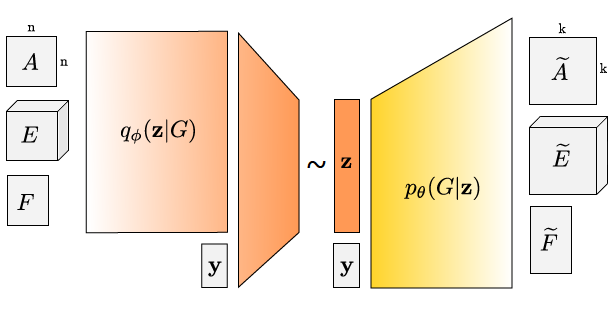
\includegraphics[width=0.75\textwidth]{data/images/SimonovskyGraphVAE.png}
    \label{fig:simonGVAE}
    \caption{Illustration of the GraphVAE architecture as presented in \cite{simonovsky_graphvae_2018}. The decoder combines graph convolutions and a MLP with concatenated labels $y$. The decoder reconstruct $\mathcal{G}$ from the latent representation and the concatenated node labels $y$.}
\end{figure}

% The encoder can either be a MLP, a GCNN or an RGCN. The same holds for the decoder with the addition that model architecture needs to be inverted. An version of a Graph VAE presented in \cite{simonovsky_graphvae_2018}. This model combines both the previous methods. The input graph undergoes relational graph convolutions before it is flattened and projected into latent space. After applying the reparametrization trick, a simple MLP decoder is used to regenerate the graph. In addition the model concatenates the input with a target vector $y$, which represents ???. The same vector is concatenated with the latent tensor. ***Elborate why they do that***.

% Reverse MLP

% Loss function

% What information can you capture when sparse compared to dense?


% Graphs can be generated recursively or in an one-shot approach. This paper uses the second approach and generates the full graph in one go. ***Cite?***
% This model will be the starting point for our research.

\subsubsection{One Shot vs. Recursive}
% One shot: MNIST vs recursive on graphs: Belli
The concept of the VAE has been used to generate data for various usecases. When using the VAE as generator, by sampling from the approximated posterior distribution $q_{\phi}\left(\mathbf{z}\right)$, we can reconstruct the data in a singular run or recursive manner.

The one shot method is the used in the popular example of the VAE generator on the MNIST dataset \cite{kingma_auto-encoding_2014}. each sample is independent from each other.

Recursive methods take part of the generated datapoint as input for the next datapoint, thus continuously generating the sample. This has been applied to generate audio and to reproduce videogame environments \cite{ha_world_2018}. In \cite{belli_image-conditioned_2019} variation of the GraphVAE has been used to recursively construct a vector roadmap, which has been presented in [link to related work].

For this thesis, we will use the one-shot method, predicting each datapoint independent from each other. The datapoints will be sparse subgraph with $n$ nodes. A single triple being $n=2$ and a subgraph representation $2<n<100$. 
% [TODO]

\subsection{Graph Matching}
\label{ssec:graphmatch}
% Intro to graph matching on sparse graphs.
In this subsection we will explain the term permutation invariance and present an algorithm to find the optimal permutation in order to match two graphs. We then derive the loss term of the graph VAE \ref{ssec:GVAE} applying the optimal matching matrix to the models prediction.

\subsubsection{Permutation Invariance}

% Permutation Invariance
% The position or rotation of a graph can vary. 
% Use graph matching to detect similarities between graphs

Permutation invariance refers to the invariance of a permutation of an object. An visual example is the the image generation of numbers. If the loss function of the model would not be permutation invariant, the generated image could show a perfect replica of the input number but being translated by one pixel the loss function would penalize the model. Geometrical permutations can be translation, scale or rotation around any axis. 

In the context of sparse graphs the most common, and relevant permutation for this thesis, is be the position of a link in the adjacency matrix. By altering its position with help of a permutation matrix, the link will connect different nodes. When matching graphs with more than two nodes, we can partially match the graphs by permuting only a subgraph instead of the full graph. This way also graphs of different sizes, can be matched. 

A model is permutation invariant, when it includes a function to detect and match such permutations between target and prediction. 


% OR: An example is in object detection in images. An object can have geometrical permutations such as translation, scale or rotation, none the less the model should be able to detect and classify it. In that case, the model is not limited by permutations and  is there fore permutation invariant.
% In our case the object is a graph and the nodes can take different positions in the adjacency matrix. To detect similarities between graphs we apply graph matching.

\subsubsection{Max-Pool Graph matching algorithm}
% These are three of the state of the art graph matching algorithms.

% \begin{itemize}
%     \item Wasserstein
%     \item Maxpooling
%     \item one more
% \end{itemize}

While there are numerous graph matching algorithms, we will focus on the max-pool algorithm, which can be effectively implement and used in the VAE setting. First presented in \cite{cho_finding_2014} in the context of computer vision and successfully trained to match graphs from feature points in an image. It uses a max-pooling graph matching approach, which is resilient to deformations and highly tolerant to outliers. The output is a reliable cost matrix. Notable is, that also graphs with different number of nodes can be matched.


% Max-pooling algorithm comes here !!!
Let us introduce a new sparse representation for a sampled subgraph, where the discrete target graph is $G=(A, E, F)$ and the continuous predicted graph $\widetilde{G}=(\widetilde{A}, \widetilde{E}, \widetilde{F})$. The $A, E, F$ are store the discrete data for the adjacency, for node attributes and the node attribute matrix of form $A \in\{0,1\}^{n \times n^{\prime}}$ with $n$ being the number of nodes in the target graph. $E\in\{0,1\}^{n \times n^{\prime} \times d_e}$ is the edge attribute matrix and a node attribute tensor of the shape $F\in\{0,1\}^{n \times d_n}$ with $d_e$ and $d_n$ being the size of the entity and relation dictionary. For the predicted graph with $k$ nodes, the adjacency matrix is $\widetilde{A} \in[0,1]^{k \times k}$, the edge attribute matrix is $\widetilde{E} \in \mathbb{R}^{k \times k \times d_{e}}$ and the node attribute matrix is $\widetilde{F} \in \mathbb{R}^{k \times d_{n}}$.


Given these graphs the algorithm aims to find the affinity matrix $S:(i, j) \times(a, b) \rightarrow \mathbb{R}^{+}$ where $i, j \in G$ and $a, b \in \widetilde{G}$. The affinity matrix expresses the similarity of all nodepairs between the two graphs and is calculated 

\begin{equation}
    \begin{array}{l}
        S((i, j),(a, b)) = \left(E_{i, j, \cdot}^{T}, \widetilde{E}_{a, b, \cdot}\right) A_{i, j} \widetilde{A}_{a, b} \widetilde{A}_{a, a} \widetilde{A}_{b, b}[i \neq j \wedge a \neq b] + \left(F_{i, \cdot}^{T} \widetilde{F}_{a, \cdot}\right) \widetilde{A}_{a, a}[i=j \wedge a=b]
    \end{array}
\end{equation}

where the square brackets define Iverson brackets \cite{simonovsky_graphvae_2018}.


The next step is to find the similarity matrix $X^* \in[0,1]^{k \times n}$. Therefore we iterate a fist-order optimization framework and get the update rule

\begin{equation}
    \mathbf{x}_{t+1} \leftarrow \frac{1}{\left\|\mathbf{S} \mathbf{x}_{t}\right\|_{2}} \mathbf{S} \mathbf{x}_{t}.
\end{equation}

To calculate $\text { Sx }$ we find the best candidate $x_{i,a}$ from the possible pairs in the affinity matrix. Heuristically, taking the argmax over all neighboring nodepair affinities yields the best result. Other options are sum-pooling or average-pooling, which do not discard potentially irrelevant information, yet have shown to perform worse. Thus, using the max-pooling approach, we can pairwise calculate

\begin{equation}
    \mathbf{Sx}_{i a}=\mathbf{x}_{i a} \mathbf{S}_{i a ; i a}+\sum_{j \in \mathcal{N}_{i}} \max _{b \in \mathcal{N}_{a}} \mathbf{x}_{j b} \mathbf{S}_{i a ; j b}.
\end{equation}

Depending on the matrix size, the number of iterations are adjusted. The resulting similarity matrix $X*$ yields a normalized probability of matching nodepairs. In order to get a discrete translation matrix, we need to find the optimal match for each node.



\subsubsection{Hungarian algorithm}

%  Find shortest path
Picking up on the nodepair probabilities $X^*$ of last chapter, we reformulate it as a linear assignment problem. Here comes into play an optimization algorithm, the so called hungarian algorithm. It original objective is to optimally assign $n$ resources to $n$ tasks. The cost of assigning task $i \in \mathbb{R}^n$ to $j \in \mathbb{R}^n$ is stored in $x_{ij}$ of the quadratic cost matrix $x \in \mathbb{R}^{n \times n}$. By assuming tasks and resources are simple nodes and taking $C=1-X^*$ we get the cost matrix $C$ for the optimal translation. This algorithm is has a complexity of $O\left(n^{4}\right)$, thus is not applicable to complete KGs but only to subgraphs with limited number of nodes per graph \cite{date_gpu-accelerated_2016}.

The core of the hungarian algorithm consist of four main steps, initial reduction, optimality check, augmented search and update. The now presented algorithm is a slight alternative of the original algorithm and improves the complexity of the update step from $O\left(n^{2}\right)$ to $O\left(n\right)$ and thus, reduces the total complexity to $O\left(n^{3}\right)$. It takes as input a bipartie graph $G=(V, U, E)$ and the cost matrix $C \in \mathbb{R}^{n \times n}$ where $V \in \mathbb{R}^n$ and $U \in \mathbb{R}^n$ are sets of nodes and $E \in \mathbb{R}^{n \times n}$ the set of edges between the nodes. The algorithm's output is a discrete matching matrix $M$. To avoid two irrelevant pages of pseudocode, the steps of the algorithm are presented in the following short summary \cite{mills2007dynamic}.

\begin{enumerate}
    \item Initialization: \\
    \begin{enumerate}
        \item Initialize the empty matching matrix $M_{0}=\emptyset$.
        \item Assign $\alpha_i$ and $\beta_i$ as follows:
        \begin{align*}
            \forall v_{i} &\in V, \quad &&\alpha_{i}=0 \\
            \forall u_{i} &\in U, \quad &&\beta_{j}=\min _{i}\left(c_{i j}\right)
        \end{align*}
        \end{enumerate}
    \item Loop $n$ times over the different stages:
    \begin{enumerate}
        \item Each unmatched node in $V$ is a root node for an Hungarian tree with when completed results in an augmentation path.
        \item Expand the Hungarian trees in the equality subgraph. Store the indices $i$ of $v_i$ encountered in the Hungarian tree in the set $I*$ and similar for $j$ in $u_j$ and the set $J^*$. If an augmentation path is found, skip the next step.
        \item Update $\alpha$ and $\beta$ to add new edges to the quality subgraph and redo the previous step.
        \begin{align*}
            \theta&=\frac{1}{2} \min _{i \in I^{*}, j \notin J^{*}}\left(c_{i j}-\alpha_{i}-\beta_{j}\right) \\
            \alpha_{i} &\leftarrow\left\{\begin{array}{ll}
            \alpha_{i}+\theta & i \in I^{*} \\
            \alpha_{i}-\theta & i \notin I^{*}
            \end{array}\right \\
            \beta_{j} &\leftarrow\left\{\begin{array}{ll}
            \beta_{j}-\theta & j \in J^{*} \\
            \beta_{j}+\theta & j \notin J^{*}
            \end{array}
        \end{align*}
        \item Augment $M_{k-1}$ by flipping the unmatched with the matched edges on the selected augmentation path. Thus $M_k$ is given by $\left(M_{k-1}-P\right) \cup\left(P-M_{k-1}\right)$ and $P$ is the set of edges of the current augmentation path.
    \end{enumerate}
    \item Output $M_n$ of the last and $n^{th}$ stage.
\end{enumerate}



\\
\subsubsection{Graph Matching VAE Loss}
Coming back to our generative model, we now explain how the loss function needs to be adjusted to work with graphs and graph matching, which results in a permutation invariant graph VAE.

The normal VAE maximizes the evidence lower-bound or, in a practical implementation, minimizes the upper-bound on negative log-likelihood. Using the notation of \ref{ssection:VAE} the graph VAE loss is

\begin{equation}
    \begin{array}{l}
    \mathcal{L}(\phi, \theta ; G)=\quad=\mathbb{E}_{q_{\phi}(\mathbf{z} \mid G)}\left[-\log p_{\theta}(G \mid \mathbf{z})\right]+\operatorname{KL}\left[q_{\phi}(\mathbf{z} \mid G) \| p(\mathbf{z})\right]
    \end{array}
\end{equation}

The loss function $\mathcal{L}$ is a combination of reconstruction term and regularization term. The regularization term is the KL divergence between a standard normal distribution and the latent space distribution of $Z$. This term does not change when adopting to graphs. The reconstruction term is the binary cross entropy between prediction and target, which in the sparse graph representation are threefold with $A, E, F$. 

% A sigmoid with logits, E,F, softmax include translation X

% r. Sigmoid activation function is used to compute
% Ae, whereas edge- and node-wise softmax is applied to obtain
% Ee and Fe, respectively. A

The predicted output of the decoder is split in three parts and while $\tilde{A}$ is activated through sigmoid, $\tilde{E}$ and $\tilde{F}$ are activated via edge- and nodewise softmax. The graph matching permutation for $A$ is applied to the target $A^{\prime}=X A X^{T}$ and for $E$ and $F$ on the prediction, $\widetilde{F}^{\prime}=X^{T} \widetilde{F}$ and $\widetilde{E}_{\cdot, \cdot, l}^{\prime}=X^{T} \widetilde{E}_{\cdot, \cdot, l} X$, $l$ being the one-hot encoded edge attribute vector which is permuted. These permuted subgraphs are then used to calculate the maximum log-likelihood estimate \cite{simonovsky_graphvae_2018}

\begin{equation}
    \begin{split}
        \log p\left(A^{\prime} \mid \mathbf{z}\right) = &1 / k \sum_{a} A_{a, a}^{\prime} \log \widetilde{A}_{a, a}+\left(1-A_{a, a}^{\prime}\right) \log \left(1-\widetilde{A}_{a, a}\right)+ \\ & +1 / k(k-1) \sum_{a \neq b} A_{a, b}^{\prime} \log \widetilde{A}_{a, b}+\left(1-A_{a, b}^{\prime}\right) \log \left(1-\widetilde{A}_{a, b}\right)
    \end{split}
\end{equation}

\begin{align}
        \log p(F \mid \mathbf{z}) &=1 / n \sum_{i} \log F_{i, \cdot}^{T} \widetilde{F}_{i,}^{\prime} \\
        \log p(E \mid \mathbf{z}) &=1 /\left(\|A\|_{1}-n\right) \sum_{i \neq j} \log E_{i, j,}^{T}, \widetilde{E}_{i, j, \cdot}^{\prime}
\end{align}

\subsection{Ranger Optimizer}

Finalizing this chapter, we introduce the novel deep learning optimizer Ranger. An optimizer, which in 2020 placed itself on the top of 12 FastAI leaderboards. Ranger combines Rectified Adam (RAdam), lookahead and optionally gradient centralization. let us shortly look into the different components.

%  REadam
RAdam is based on the popular adam optimizer. It improves the learning by dynamically rectifying Adam's adaptive momentum. This is done by reducing the variance of the momentum, which is especially large at the beginning of the training. Thus, leading to a more stable and accelerated start \cite{liu_variance_2020}.

The Lookahead optimizer was inspired by recent advances in the understanding of loss surfaces of deep neural networks, thus proposes an approach where, a second optimizer 'looks ahead' on a set of parallel trained weights. while the computation and memory cost are negligible, it learning improves and the variance of the main optimizer is reduced \cite{zhang_lookahead_2019}.

The last and most novel optimization technique, Gradient Centralization, acts directly on the gradient by normalizing it to a zero mean. Especially on convolutional neural networks, this helps regularizing the gradient and boosts learning. This method can be added to existing optimizers and can be seen as constrain of the loss function \cite{yong_gradient_2020}.

Concluding we can say that Ranger is a state of the art deep learning optimizer with accelerating and stabilizing properties, incorporating three different optimization methods, which synergize with each other. Considering that generative models are especially unstable during training, we see Ranger as a good fit for this research.



% LookAhead was inspired by recent advances in the understanding of loss surfaces of deep neural networks, and provides a breakthrough in robust and stable exploration during the entirety of training.